\title{Rokko tutorial}

\errorcontextlines=5

\newtheorem{rei}{Example}
\renewcommand{\therei}{}

\AtBeginSection[]{
    \begin{frame}
        \tableofcontents[currentsection]
    \end{frame}
}

\begin{document}

\lstset{language=c++,basicstyle=\ttfamily\tiny,showspaces=false,keepspaces=true,rulecolor=\color[cmyk]{0, 0.29,0.84,0}}

\begin{frame}
  \titlepage
  \noindent {\footnotesize PDF file: \url{http://sf.net/projects/rokko-tutorial/files/}} \\
  \noindent {\footnotesize LaTeX source: \url{http://github.com/cmsi/rokko-tutorial/}}
\end{frame}

%% \section*{Outline}
%% \begin{frame}
%%   \tableofcontents
%% \end{frame}

\section{Overview of Rokko tutorial}

%% \begin{frame}{Rokkoチュートリアル スタッフ}
%%   \begin{itemize}
%%   \item 講師
%%     \setlength{\itemsep}{1em}
%%     \begin{itemize}
%%       \setlength{\itemsep}{1em}
%%     \item 坂下達哉 (東大物性研) \ \href{mailto:t-sakashita@issp.u-tokyo.ac.jp}{t-sakashita@issp.u-tokyo.ac.jp}
%% %    \item 藤堂眞治 (東大院理/物性研) \ \href{mailto:wistaria@phys.s.u-tokyo.ac.jp}{wistaria@phys.s.u-tokyo.ac.jp}
%% %    \item 五十嵐 亮 (東大物性研) \ \href{mailto:rigarash@issp.u-tokyo.ac.jp}{rigarash@issp.u-tokyo.ac.jp}
%% %    \item 本山裕一 (東大物性研) \ \href{mailto:y-motoyama@issp.u-tokyo.ac.jp}{y-motoyama@issp.u-tokyo.ac.jp}
%%     \end{itemize}
%%   \item 主催
%%     \begin{itemize}
%%     \item CMSI: Computational Materials Science Initiative \url{http://cms-initiative.jp/}
%%     \end{itemize}
%%   \end{itemize}
%% \end{frame}

\begin{frame}
  \frametitle{Contents of the tutorail}
  \begin{itemize}
    %\setlength{\itemsep}{1em}
  \item lecture: Existing eigenvalue algorithms \& solvers / Linear algebra solvers
  \item lecture: Overview of Rokko and its structure
%  \item hands-on: Rokkoのインストール
  \item lecture/hands-on: Structure of sequential dense solvers / Running sample programs
  \item lecture/hands-on: Structure of MPI parallelized dense solvers / Running sample programs
  \item lecture/hands-on: Structure of sequential sparse solvers / Running sample programs
  \item hands-on: sample programs of diagonalization for quantum spin systems
%  \item 実習: TITPACK2へのRokko組み込み実習
%  \item 実習: アプリケーションからのRokkoの利用
%  \item (付録: ALPS/Baristaパッケージ)
 % \item (付録: MateriAppsとMateriApps LIVE!)
  \end{itemize}
\end{frame}


\section{Eigenvalue Algorithms / Solvers, Linear Algebra Libraries}

\begin{frame}
  \frametitle{Existing eigenvalue algorithms \& solvers / Linear algebra solvers}
  \begin{itemize}
    \setlength{\itemsep}{1em}
  \item Diagonalization of matrix
  \item Eigenvalue algorithms
  \item Existing eigenvalue solvers / Linear algebra libraries
  \end{itemize}
\end{frame}

\begin{frame}
  \frametitle{Matrix diagonalization}
  \begin{itemize}
    %\setlength{\itemsep}{1em}
  \item Matrix type
    \begin{itemize}
    \item real symmetric matrix, real unsymmetric matrix, complex Hermitean matrix, complex non-Hermitean matrix
    \end{itemize}
  \item Type of matrix storage
    \begin{itemize}
      \item dense matrix, CRS (Compressed Row Storage) format, MatFree\\
            (corresponding to ``small'', ``middle'', ``large'' in TITPACK2 resp.)
    \end{itemize}
  \item Eigenvalues to be computed
    \begin{itemize}
      \item all or the greatest (least) ones in absolute value, ones in some region
    \end{itemize}
  \item Eigenvectors
    \begin{itemize}
      \item wanted/unwanted
    \end{itemize}
  \end{itemize}
\end{frame}

\begin{frame}
  \frametitle{Definitions of Terms}
  \begin{itemize}
    %\setlength{\itemsep}{1em}
  \item Eigenvalue algorithm
%    \begin{itemize}
%      \item 固有値問題を解くためのアルゴリズム
%    \end{itemize}
  \item Eigensolver (solver for eigenvalue problem)
    \begin{itemize}
      \item Implementation of eigenvalue algorithm
    \end{itemize}
  \item Eigensolver Library
    \begin{itemize}
      \item a library which consists of only eigensolvers
    \end{itemize}
  \item Linear Algebra Library
    \begin{itemize}
      \item collection of eigensolvers and other solvers
    \end{itemize}
  \item Exact diagonalization package
    \begin{itemize}
      \item Software to deal with eigenvalue problems of Hamiltonian matrix for the quantum lattice model
    \end{itemize}
  \end{itemize}
\end{frame}

\begin{frame}
  \frametitle{Eigenvalue algortihm (part)}
  \begin{itemize}
    %\setlength{\itemsep}{1em}
  \item Eigenvalue algorithms for tridiagonalized matrix
    \begin{itemize}
      \item bisection method, QR method, MR3 method, divide-conquer method+QR method
    \end{itemize}
  \item Direct diagonalization of dense matrix
    \begin{itemize}
      \item Jacobi method
    \end{itemize}
  \item Tridiagonalization of dense matrix
    \begin{itemize}
      \item Householder method
    \end{itemize}
  \item Direct diagonalization of sparse matrix
    \begin{itemize}
      \item power method, inverse power method, Rayleigh quotient iteration method, Jacobi-Davidson method, LOBPCG, Krylov-Schur method
    \end{itemize}
  \item Tridiagonalization of sparse matrix
    \begin{itemize}
      \item Lanczos method, Arnoldi method, Restart Lanczos, Thick-restart Lanczos method
    \end{itemize}
  \item Other methods
    \begin{itemize}
      \item Sakurai-Sugiura method
    \end{itemize}
  \end{itemize}
\end{frame}

\begin{frame}
  \frametitle{Eigenvalue Algothims}
  \begin{center}
    \includegraphics[height=0.45\textheight]{figure/AppliedNumericalLinearAlgebra.jpg} \ \
    \includegraphics[height=0.45\textheight]{figure/TheSymmetricEigenvalueProblem.jpg} \ \
    \includegraphics[height=0.45\textheight]{figure/SenkeikeisanNoSuri.jpg}  \ \
    \includegraphics[height=0.45\textheight]{figure/GyoretsuNoKoyuchi.jpg}
  \end{center}
\end{frame}

\begin{frame}
  \frametitle{Existing eigesolver libraries (for dense matrix)}
  \begin{itemize}
    %\setlength{\itemsep}{1em}
  \item \href{http://www.aics.riken.jp/labs/lpnctrt/EigenExa.html}{EigenExa}: dense solver
    \begin{itemize}
      \item Householder (tri-diagonalization, penta-diagonalization) + divide\&conquer + QR
    \end{itemize}
  \item \href{http://elpa.rzg.mpg.de}{ELPA}
    \begin{itemize}
      \item Householder + divide\&conquer method + QR
    \end{itemize}
  \end{itemize}
\end{frame}

\begin{frame}
  \frametitle{Existing eigesolver libraries (for sparse matrix)}
  \begin{itemize}
  \item \href{http://trilinos.org/packages/anasazi/}{Anasazi}: Mainly iteration solvers
    \begin{itemize}
      \item Krylov-Schur, Jacobi-Davidson, XXX-Davidson, LOBPCG, Implicit Riemannian Trust Region Method
    \end{itemize}
  \item \href{http://www.caam.rice.edu/software/ARPACK/}{ARPACK}
    \begin{itemize}
      \item Implicit Restarted Lanczos
    \end{itemize}
  \item \href{https://code.google.com/p/blopex/}{BLOPEX}
    \begin{itemize}
    \item Locally Optimal Block Preconditioned Conjugate Gradient Method (LOBPCG)
    \end{itemize}
  \item \href{http://www.grycap.upv.es/slepc/}{SLEPc}: Mainly iteration solvers, Need to select seq or MPI parallel in building time
    \begin{itemize}
      \item Krylov-Schur, Generalized Davidson, Jacobi-Davidson, Rayleigh Quotient Conjugate Gradient, Contour integral Sakurai-Sugiura, Power method, Subspace Itertation, Arnoldi (explicit restart), Lanczos (explicit restart) \\
    \end{itemize}
  \item \href{http://www.comp-phys.org/software/ietl/}{IETL}: iterative solvers included in ALPS
    \begin{itemize}
      \item Lanczos, etc.
    \end{itemize}
  \end{itemize}
\end{frame}

\begin{frame}
  \frametitle{Existing eigesolver libraries (for dense matrix)}
  \begin{itemize}
    %\setlength{\itemsep}{1em}
  \item Vendor's implementation of LAPACK and ScaLAPACK
    \begin{itemize}
    \item \href{https://developer.apple.com/library/mac/documentation/Performance/Conceptual/vecLib/Reference/reference.html}{Apple VecLib}: LAPACK
    \item Fujitsu SSLII: LAPACK, a part of ScaLAPACK(part), etc.
    \item \href{https://software.intel.com/en-us/mkl_11.1_ref}{Intel MKL}: LAPACK, ScaLAPACK
    \item
      \href{http://developer.amd.com/tools-and-sdks/cpu-development/amd-core-math-library-acml/}{ACML(AMD
        Core Math Library)}: LAPACK
    \item \href{http://www.openblas.net}{OpenBLAS}: BLAS + a part of LAPACK routines(sucessive implementation for GotoBLAS)

    \end{itemize}
  \item \href{http://www.netlib.org/lapack/}{Netlib LAPACK}: LAPACKのreference implementation
    \begin{itemize}
      \item Householder+QR, Householder + divide\&conquer + QR, Householder+bisection method, Householder+MR3
    \end{itemize}
  \item \href{http://www.netlib.org/scalapack/}{Netlib ScaLAPACK}: reference implmentation of ScaLAPACK
    \begin{itemize}
      \item Householder + QR, Householder + divide\&conquer + QR, Householder+bisection, Householder + MR3
    \end{itemize}
  \item \href{http://eigen.tuxfamily.org/}{Eigen3}(sequential, thread parallelized for matrix-matrix product)
    \begin{itemize}
      \item Householder+QR
    \end{itemize}
  \item \href{http://libelemental.org}{Elemental}:included eigensolvers ''MRRR'' works well, only for square processes.
    \begin{itemize}
      \item Householder+MR3
    \end{itemize}
  \end{itemize}
\end{frame}

\begin{frame}
  \frametitle{Existing eigesolver libraries (for sparse matrix)}
  \begin{itemize}
    %\setlength{\itemsep}{1em}
  \item \href{http://trilinos.org}{Trilinos}: It includes eigensolvers Anasazi.
  \item Xabclib (\href{http://ppopenhpc.cc.u-tokyo.ac.jp/}{ppOpen AT})
  \end{itemize}
\end{frame}

\begin{frame}
  \frametitle{Recommnded order}
  \begin{itemize}
    %\setlength{\itemsep}{1em}
  \item For dense matrix (seq.)
    \begin{itemize}
      \item LAPACK (vendor impl.) $>$ Eigen3
    \end{itemize}
  \item For dense matrix (MPI)
    \begin{itemize}
      \item EigenExa $>$ ELPA $>$ ScaLAPACK (vendor impl.) $>$ Elemental
    \end{itemize}
  \item For sparse matrix (seq. MPI)
    \begin{itemize}
      \item Anasazi $>$ SLEPc
    \end{itemize}
  \end{itemize}
\end{frame}

\begin{frame}
  \frametitle{Latestest eigensolvers}
  \begin{itemize}
    \setlength{\itemsep}{1em}
  \item There are several hybrid parallized(MPI+OpenMP) eigensolvers.
  \item It’s almost impossible for users to implement parallel eigensolvers by themselves.
  \item Utilize open source hybrid parallelized eigensolvers.
  \end{itemize}
\end{frame}

\begin{frame}
  \frametitle{Exact diagonalization package}
  \begin{itemize}
    \setlength{\itemsep}{1em}
  \item Popular packages
    \begin{itemize}
    \item ALPS (\href{http://alps.comp-phys.org/static/software/applications/diag/fulldiag/doc/}{fulldiag} / \href{http://alps.comp-phys.org/mediawiki/index.php/Documentation:sparsediag}{sparsediag}): It uses LAPACK, IETL.
    \item \href{http://quattro.phys.sci.kobe-u.ac.jp/Kobe_Pack/Kobe_Pack.html}{KOBEPACK}: It includes their own eigensolvers
    \item \href{http://www-e.uni-magdeburg.de/jschulen/spin/}{SPINPACK}: It use LAPACK
    \item \href{http://www.noc.titech.ac.jp/~phys0016_nishimori/titpack2_new/index-e.html}{TITPACK2}: It includes their own eigensolvers
    \end{itemize}
  \item sequential or thread parallized, no MPI parallelized.
  \item It makes calculations for a large number of sites difficult.
  \end{itemize}
\end{frame}

\section{Rokkoの概要と内部構造}

\begin{frame}
  \frametitle{Overview and Structure of Rokko}
  \begin{itemize}
    \setlength{\itemsep}{1em}
  \item Problems in using existing eigensolvers
  \item Overview of Rokko
  \item 並列ソルバの基本概念
  \item Rokkoの内部構造
  \end{itemize}
\end{frame}

\begin{frame}
  \frametitle{Problems in using existing eigensolvers}
  \begin{itemize}
    \setlength{\itemsep}{1em}
  \item Different designs (interface, block size, padding...) for different eigensolvers
  \item Documentation is insufficient.
  \item Different compiling / link options depending on architectures
  \item Linking problems between languages C++ / C / Fortran
  \item Complicated dependency among lower level libraries
  \item Users want rough estimate for performace of eigensolvers before trying it.
  \end{itemize}
\end{frame}

\begin{frame}
  \frametitle{Dependency of parallel dense solvers}
  \begin{center}
    \includegraphics[height=0.8\textheight]{figure/eigensolver_dependency.pdf}
  \end{center}
\end{frame}

\begin{frame}
  \frametitle{Delvelopers of Rokko}
  \begin{itemize}
    \setlength{\itemsep}{1em}
  \item Tatsuya Sakashita (ISSP, Tokyo Univ.) \ \href{mailto:t-sakashita@issp.u-tokyo.ac.jp}{t-sakashita@issp.u-tokyo.ac.jp}
  \item Yuichi Motoyama (ISSP, Tokyo Univ.) \ \href{mailto:y-motoyama@issp.u-tokyo.ac.jp}{y-motoyama@issp.u-tokyo.ac.jp}
  \item Ryo Igarashi (ISSP, Tokyo Univ.) \ \href{mailto:rigarash@issp.u-tokyo.ac.jp}{rigarash@issp.u-tokyo.ac.jp}
  \item Tsuyoshi Okubo (ISSP, Tokyo Univ.) \ \href{mailto:t-okubo@issp.u-tokyo.ac.jp}{t-okubo@issp.u-tokyo.ac.jp}
  \item Synge Todo (Department of Physics / ISSP, Tokyo Univ.) \ \href{mailto:wistaria@phys.s.u-tokyo.ac.jp}{wistaria@phys.s.u-tokyo.ac.jp}
  \end{itemize}
\end{frame}

\begin{frame}
  \frametitle{Overview of Rokko}
  \begin{itemize}
    %\setlength{\itemsep}{1em}
  \item Language
    \begin{itemize}
      %\setlength{\itemsep}{1em}
    \item Core parts: C++
    \item Language binding: C, Fortran90
    \item Benchmarking script: Python
    \end{itemize}
  \item License
    \begin{itemize}
      %\setlength{\itemsep}{1em}
    \item Boost licene (almost freely available)
    \end{itemize}
  \item Source code
    \begin{itemize}
      %\setlength{\itemsep}{1em}
    \item Open to the public by GitHub\\
          \url{https://github.com/t-sakashita/rokko/}
    \end{itemize}
  \end{itemize}
\end{frame}

\begin{frame}
  \frametitle{Management of source code by VCS (Version Control System)}
  \begin{itemize}
  \item 開発者が複数になると, ディレクトリ名やログファイルによるバージョン管理はすぐに破綻する
  \item ソースコードをサーバー上で一括管理
    \begin{itemize}
    \item ネットワーク経由でソースを check out/check in
    \end{itemize}
  \item 全ての修正履歴を保存
  \item 複数人が同時に更新した場合に衝突を回避するしくみ
  \item ブランチ・マージ・タグ付けなどが可能
  \item 開発者が一人, 公開の予定がない場合でも積極的に使うべき
  \item 参考資料: バージョン管理web講習会 {\tiny
      \url{http://www.cms-initiative.jp/ja/research-support/develop-support/how-to-publish/develop-apps/dt0l33}}
  \end{itemize}
\end{frame}

\begin{frame}
  \frametitle{Design Policy of Rokko}
  \begin{itemize}
    \setlength{\itemsep}{1em}
  \item Common vector and matrix class
  \item Absorb differences of indivisual solvers by wrappers
    \begin{itemize}
      %\setlength{\itemsep}{1em}
    \item As eigensolvers develop and change, we modify wrapping functions to keep Rokko's interface the same.
    \end{itemize}
  \item Without recompiling Rokko, you can select solver in runtime.
  \item Multiple solvers can be called at one program.
  \item Less overhead wrappers by using virutal functions and templates
  \item Available from C++, C, Fortran90
  \end{itemize}
\end{frame}

\begin{frame}
  \frametitle{Components of Rokko}
  \begin{itemize}
    %\setlength{\itemsep}{1em}
  \item Install scripts for eigenvalue solvers / linear algebra libraries
  \item Common fundamental class (distributed matrix, process grid, etc.)
  \item Wrappers for eigensolvers (in C++)
  \item Factory for eigensolvers (in C++)
  \item C/Fortran wrapper
  \item Test/sample programs
  \item Benchmark scripts (future work)
  \end{itemize}
\end{frame}

\begin{frame}
  \frametitle{Rokko Software Stack}
  \begin{center}
    \includegraphics[height=0.8\textheight]{figure/rokko-software-stack.jpg}
  \end{center}
\end{frame}

\section{Install Rokko}

\begin{frame}
  \frametitle{Required tools and libraries to install Rokko}
  \begin{itemize}
    \setlength{\itemsep}{1em}
  \item CMake: \url{http://www.cmake.org}
  \item Boost C++ Libraries: \url{http://www.boost.org}
  \item Install scripts: \url{https://github.com/wistaria/installer}
  \item Lists of installation for primary supercomputer in Japan \\
    \url{https://github.com/wistaria/installer/wiki}
  \end{itemize}
\end{frame}

\begin{frame}
  \frametitle{Building system: CMake}
  \begin{itemize}
    \setlength{\itemsep}{1em}
  \item Utility to generate Makefile.\\
  It is intended to be next-generation autoconf / automake.
    \begin{itemize}
    \item It can generate Visual C++ solution file for Windows and Xcode project file for Mac OS X.
    \end{itemize}
  \item The setting for source code is described in CMakeLists.txt
  \item It has an integrated test (CTest) and binaray distribution (CPack).
  \item Automatic detection of dependency of source files
  \item Separation of source and build directories. (It makes version control easy)
  \end{itemize}
\end{frame}

\begin{frame}
  \frametitle{Installing Third-party eigensolvers / linear algebra libraries}
  \begin{itemize}
    \setlength{\itemsep}{1em}
  \item Eigen3 (this vector and matrix class is utilized in Rokko), LAPACKE (C interface of LAPACK) $\rightarrow$ They are bundled in Rokko.
  \item Install scripts: \href{https://github.com/t-sakashita/rokko/tree/master/3rd-party/install}{3rd-party/install}
    \begin{itemize}
      \item Eigensolver libraries: Anasazi, EigenExa, Elemental, ELPA, PETSc, ScaLAPACK, SLEPc
      \item Available architectures: K/FX10, x86 supercomputer/cluster (Intel compiler/GCC), Mac OS X (GCC), etc.
    \end{itemize}
  \item These solvers were already installed in primary supercomputers in Japan: \url{https://github.com/t-sakashita/rokko/wiki/PreInstall}
  \end{itemize}
\end{frame}

\begin{frame}[c,fragile]
  \frametitle{Install Rokko}
  \begin{itemize}
    %\setlength{\itemsep}{1em}
  \item Set environment variables (for phi.aics.riken.jp)
\begin{lstlisting}[style=shstyle]
source /opt/nano/alps/alpsvars.sh
\end{lstlisting}
  \item Download and decompress source codes
\begin{lstlisting}[style=shstyle]
cd $HOME
wget --no-check-certificate https://github.com/t-sakashita/rokko/archive/0.2.tar.gz \
 -O rokko-0.2.tar.gz
tar zxvf rokko-0.2.tar.gz
\end{lstlisting}
  \item Run CMake
%\begin{lstlisting}[style=shstyle]
%cmake $HOME/rokko-0.2 -DBoost_ROOT_DIR=/opt/local/boost_1_55_0 -DCMAKE_BUILD_TYPE=Debug -DCMAKE_CXX_COMPILER=icpc -DCMAKE_C_COMPILER=icc -DCMAKE_Fortran_COMPILER=ifort -DOpenMP_CXX_FLAGS=-openmp -DOpenMP_C_FLAGS=-openmp -DROKKO_SOLVER_DIR=/opt/nano/rokko -DSCALAPACK_LIB="-lmkl_scalapack_lp64 -lmkl_blacs_intelmpi_lp64 -mkl=parallel" -DCMAKE_INSTALL_PREFIX=$HOME/rokko_install
%\end{lstlisting}
\begin{lstlisting}[style=shstyle]
mkdir rokko-build
cd rokko-build

cmake $HOME/rokko-0.2 \
 -DBoost_ROOT_DIR=/opt/local/boost_1_55_0 \
 -DCMAKE_BUILD_TYPE=Debug \
 -DCMAKE_CXX_COMPILER=icpc -DCMAKE_C_COMPILER=icc -DCMAKE_Fortran_COMPILER=ifort \
 -DOpenMP_CXX_FLAGS=-openmp -DOpenMP_C_FLAGS=-openmp \
 -DROKKO_SOLVER_DIR=/opt/nano/rokko \
 -DSCALAPACK_LIB="-lmkl_scalapack_lp64 -lmkl_blacs_intelmpi_lp64 -mkl=parallel" \
 -DCMAKE_INSTALL_PREFIX=$HOME/rokko_install
\end{lstlisting}
  \end{itemize}
\end{frame}

\begin{frame}[c,fragile]
  \frametitle{Installing Rokko (cont.)}
  \begin{itemize}
  \item If you can't copy and paste the above, use the following script:
\begin{lstlisting}[style=shstyle]
cp /home/hands-on/rokko_20140918/cmake-rokko.sh  .
bash ./cmake-rokko.sh
\end{lstlisting}
  \item Make, test, and install
\begin{lstlisting}[style=shstyle]
make -j 10
make test
make install
\end{lstlisting}
  \end{itemize}
\end{frame}

\begin{frame}[c,fragile]
  \frametitle{Verification of installation}
Display a list of available eigensolvers in Rokko \RokkoFilename{tool/rokko_solvers.cpp}
\begin{lstlisting}[style=shstyle]
cd rokko/tool
./rokko_solvers
\end{lstlisting}

Output result
\begin{lstlisting}[style=shstyle]
[serial dense solvers]
  eigen3
  lapack
[parallel dense solvers]
  eigen_exa_s
  eigen_exa_sx
  scalapack
  scalapack_pdsyevd
[parallel sparse solvers]
  anasazi
  slepc
\end{lstlisting}

\end{frame}

\begin{frame}[c,fragile]
  \frametitle{Directory structure of Rokko}

\dirtree{%
 .1 \RokkoFilename{}.
 .2 \RokkoFilename{rokko}
 $\cdots$ Rokko body (header \& source files).
 .2 \RokkoFilename{sample}
 $\cdots$ Sample programs in C++.
 .3
 \href{https://github.com/t-sakashita/rokko/tree/develop/sample/dense}{dense}
 $\cdots$ for dense matrix (seq\. \& MPI).
 .3 \href{https://github.com/t-sakashita/rokko/tree/develop/sample/sparse}{sparse} $\cdots$ for sparse matrix (MPI).
 .2 \href{https://github.com/t-sakashita/rokko/tree/develop/sample_c}{sample_c} $\cdots$ Sample programs in C.
 .3 \href{https://github.com/t-sakashita/rokko/tree/develop/sample_c/dense}{dense} $\cdots$ for dense matrix (seq\. \& MPI).
 .3
 \href{https://github.com/t-sakashita/rokko/tree/develop/sample_c/sparse}{sparse}
 $\cdots$ spapse matrix (MPI).
 .2 \href{https://github.com/t-sakashita/rokko/tree/develop/sample_fortran}{sample_fortran}
 $\cdots$ Sample programs in Fortran.
 .3 \href{https://github.com/t-sakashita/rokko/tree/develop/sample_fortran/dense}{dense} $\cdots$ dense (seq\.\&MPI).
 .3 \href{https://github.com/t-sakashita/rokko/tree/develop/sample_fortran/sparse}{sparse} $\cdots$ sparse matrix (MPI).
% .2
% \href{https://github.com/t-sakashita/rokko/tree/develop/test}{test}
% $\cdots$ ctest用(インストール成否の確認).
% .2 3rd-party $\cdots$ 固有値ソルバ.
 .2 \href{https://github.com/t-sakashita/rokko/tree/develop/tutorial}{tutorial} $\cdots$ Tutorial.
 .3
 \href{https://github.com/t-sakashita/rokko/tree/develop/tutorial/titpack}{titpack}
 $\cdots$ Gradually rewriting TITPACK2 to use Rokko.
}

\end{frame}

\section{Parallel sequentail solvers}

\subsection{Specification of Rokko interface}

\begin{frame}[c,fragile]
  \frametitle{rokko::localized\_matrix class template}
  \begin{itemize}
  \item \RokkoFilename{rokko/localized_matrix.hpp}
\begin{lstlisting}
namespace rokko {
template<typename MATRIX_MAJOR = rokko::matrix_row_major>
class localized_matrix {
public:
  typedef MATRIX_MAJOR major_type;
  localized_matrix();
  localized_matrix(int rows, int cols);
  template <typename T>
  localized_matrix(T const& other);
  template <typename T>
  matrix_type& operator=(T const& other);
  double operator[](int i, int j) const;
  double& operator[](int i, int j);
  int get_m_global() const;
  int get_n_global() const;
  int get_m_local() const;
  int get_n_local() const;
  bool is_gindex_myrow(const int& global_i) const;
};
}
\end{lstlisting}
  \end{itemize}
\end{frame}

\begin{frame}[c,fragile]
  \frametitle{Usage example of rokko::localized\_vector and rokko::localized\_matrix}
  \begin{itemize}
  \item \RokkoFilename{test/localized\_matrix.cpp}
\begin{lstlisting}
int dim = 3;
rokko::localized_matrix<> M(dim,dim);
M << 1,2,3,4,5,6,7,8,9;
double a = 5.0;
rokko::localized_vector u(dim);
u << 1,2,3;
rokko::localized_vector v(dim);
v << 4,5,6;
rokko::localized_vector w = a*u+M*v;
\end{lstlisting}
  \end{itemize}
\end{frame}

\begin{frame}[c,fragile]
  \frametitle{rokko::serial\_dense\_solver class}
  \begin{itemize}
    %\setlength{\itemsep}{1em}
  \item Initialize the solver
\begin{lstlisting}
rokko::serial_dense_solver solver(name);
solver.initialize(argc, argv);
\end{lstlisting}
  \item Finalize the solver
\begin{lstlisting}
solver.finalize();
\end{lstlisting}
  \item Diagonalize a dense matrix (the matrix will be overwritten)
\begin{lstlisting}
rokko::localized_matrix<matrix_col_major> mat(dim, dim, solver);
...
rokko::localized_vector evals(dim);
rokko::localized_matrix<matrix_col_major> evecs(dim, dim, solver);
solver.diagonalize(mat, evals, evecs);
\end{lstlisting}
%  \item 登録されているソルバの一覧
%\begin{lstlisting}
%std::vector<std::string> names = rokko::serial_dense_solver::solvers();
%\end{lstlisting}
  \end{itemize}
\end{frame}

\subsection{Sample programs}

\begin{frame}[c,fragile]
  \frametitle{Sample for diagonalization}
  \begin{itemize}
    %\setlength{\itemsep}{1em}
%  \item 逐次密行列ソルバーの一覧 \href{https://github.com/t-sakashita/rokko/blob/master/test/serial_dense_solvers.cpp}{test/serial\_dense\_solvers.cpp}
%\begin{lstlisting}[style=shstyle]
%./test/serial_dense_solvers
%\end{lstlisting}
  \item Using dsyev in LAPACK directyly \RokkoFilename{sample/dense/dsyev.cpp}
\begin{lstlisting}[style=shstyle]
./sample/dense/dsyev
\end{lstlisting}
Using seq. dense solvers
  \item C++ ver. \RokkoFilename{sample/dense/frank.cpp}
\begin{lstlisting}[style=shstyle]
./sample/dense/frank lapack 5
\end{lstlisting}
  \item C ver. \RokkoFilename{sample_c/dense/frank.c}
\begin{lstlisting}[style=shstyle]
./sample_c/dense/frank lapack 5
\end{lstlisting}
  \item Fortran ver. \RokkoFilename{sample_c/dense/frank.f90}
\begin{lstlisting}[style=shstyle]
./sample_fortran/dense/frank lapack 5
\end{lstlisting}
  \end{itemize}
\end{frame}

\section{Parallel MPI eigensolvers}

\subsection{Basic concepts}

\begin{frame}
  \frametitle{2D process grid}
  \begin{itemize}
    %\setlength{\itemsep}{1em}
  \item Assigning MPI processes in 2-dimension
  \item Two types of majors: row-major / column-major
  \item Example: 4 processes (no. {\color{blue}0,1,2,3})
%  \begin{center}
%    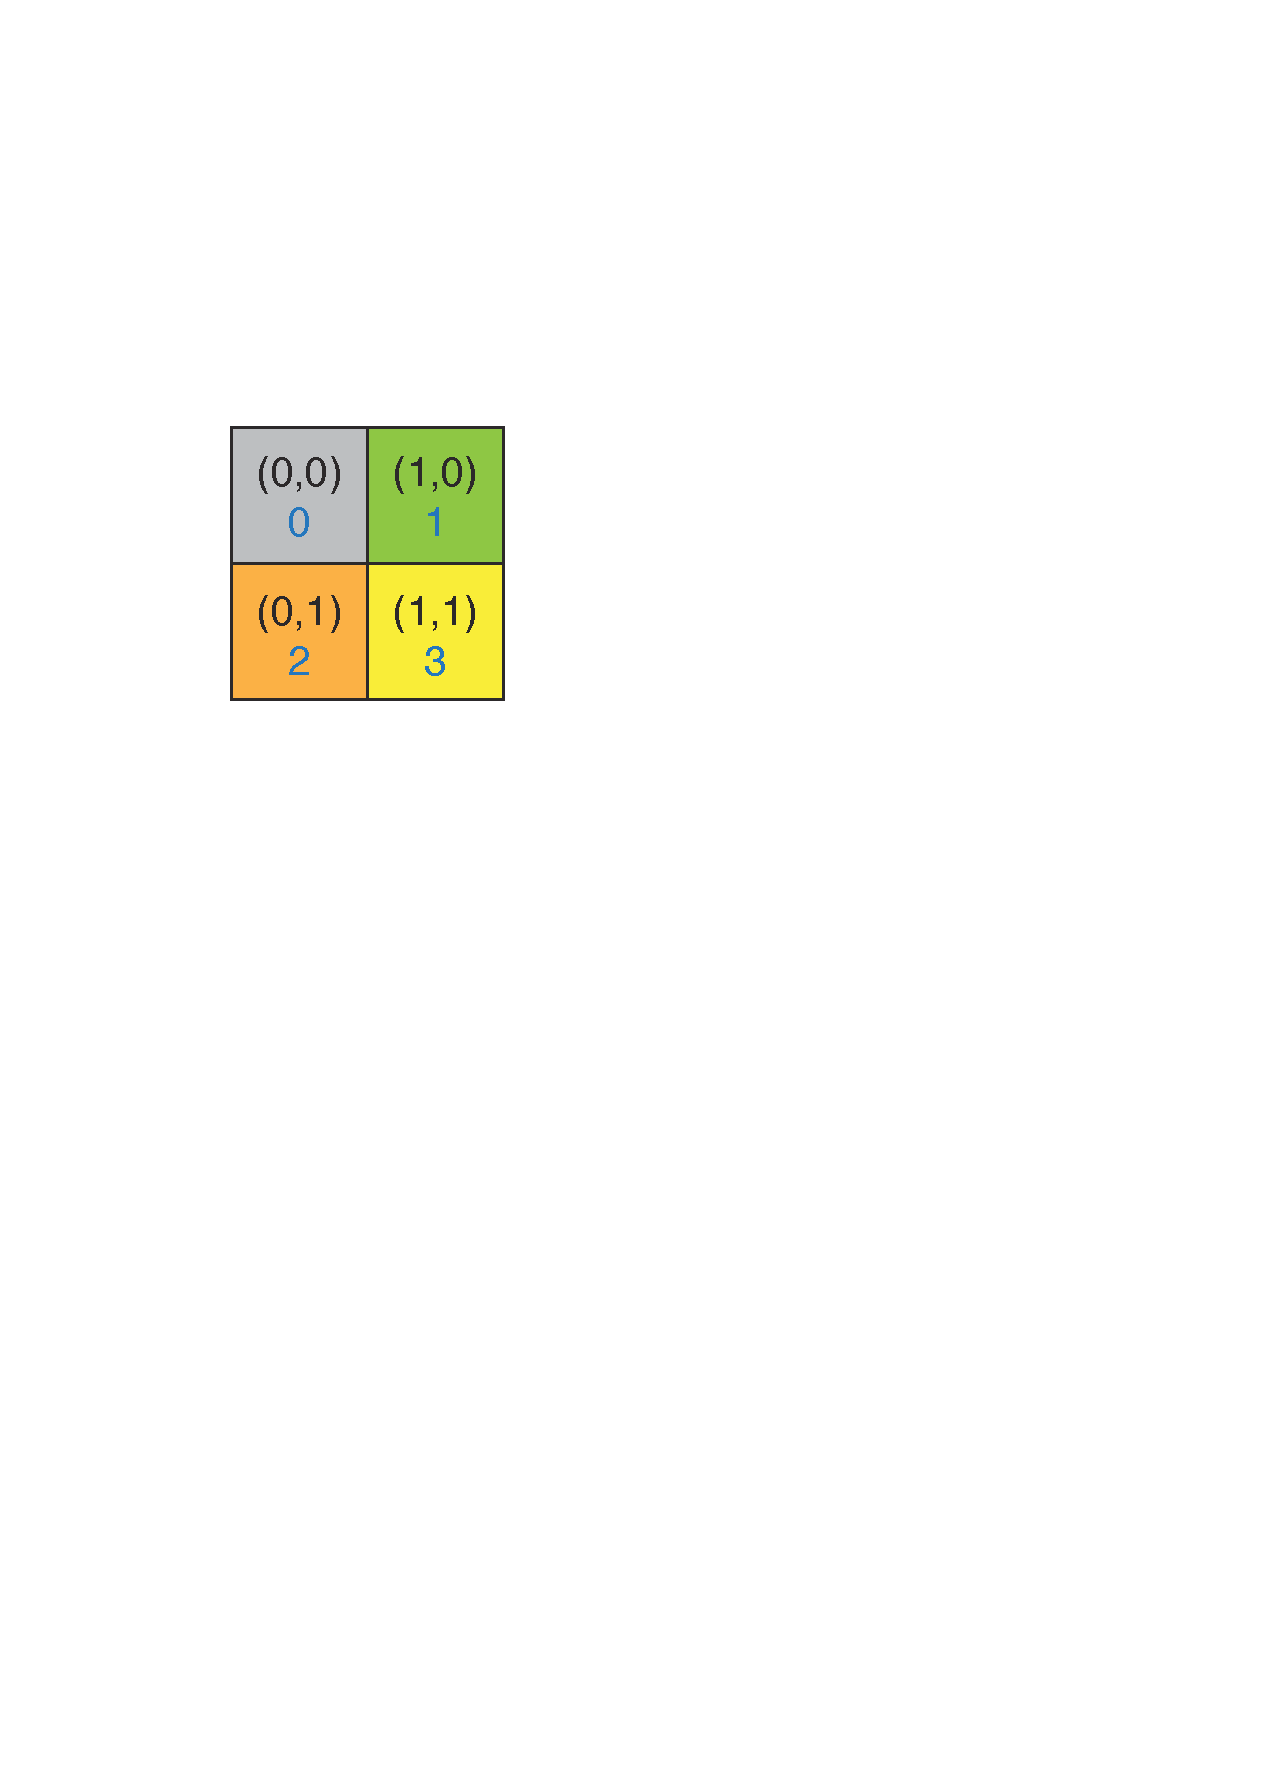
\includegraphics[height=0.25\textheight]{figure/grid-row-major.pdf} \ \ \ \
%    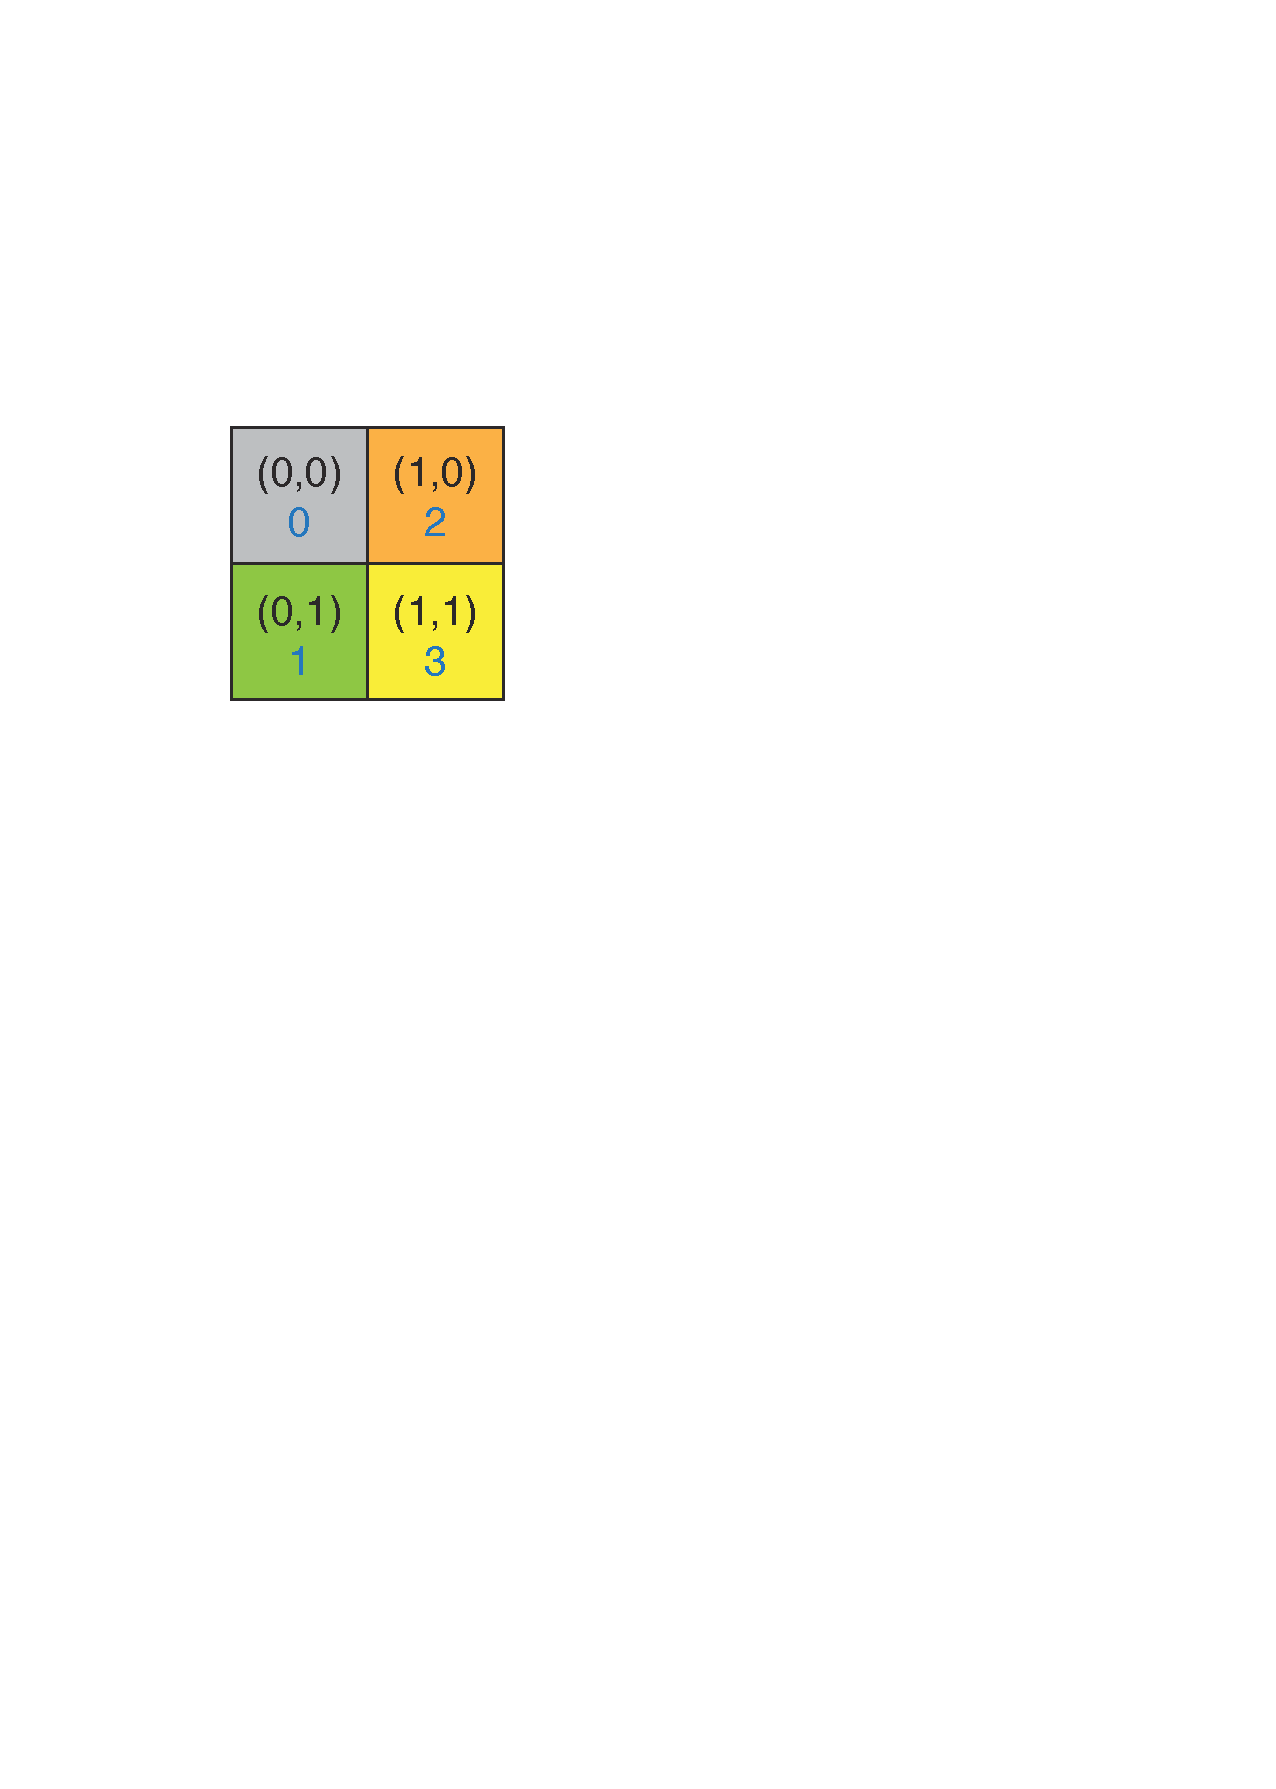
\includegraphics[height=0.25\textheight]{figure/grid-column-major.pdf}\\
%  (left:row-major, right:column-major)
%  \end{center}
  \begin{figure}[htbp]
\begin{tabular}{cc}
\begin{minipage}{0.4\hsize}
\begin{center}
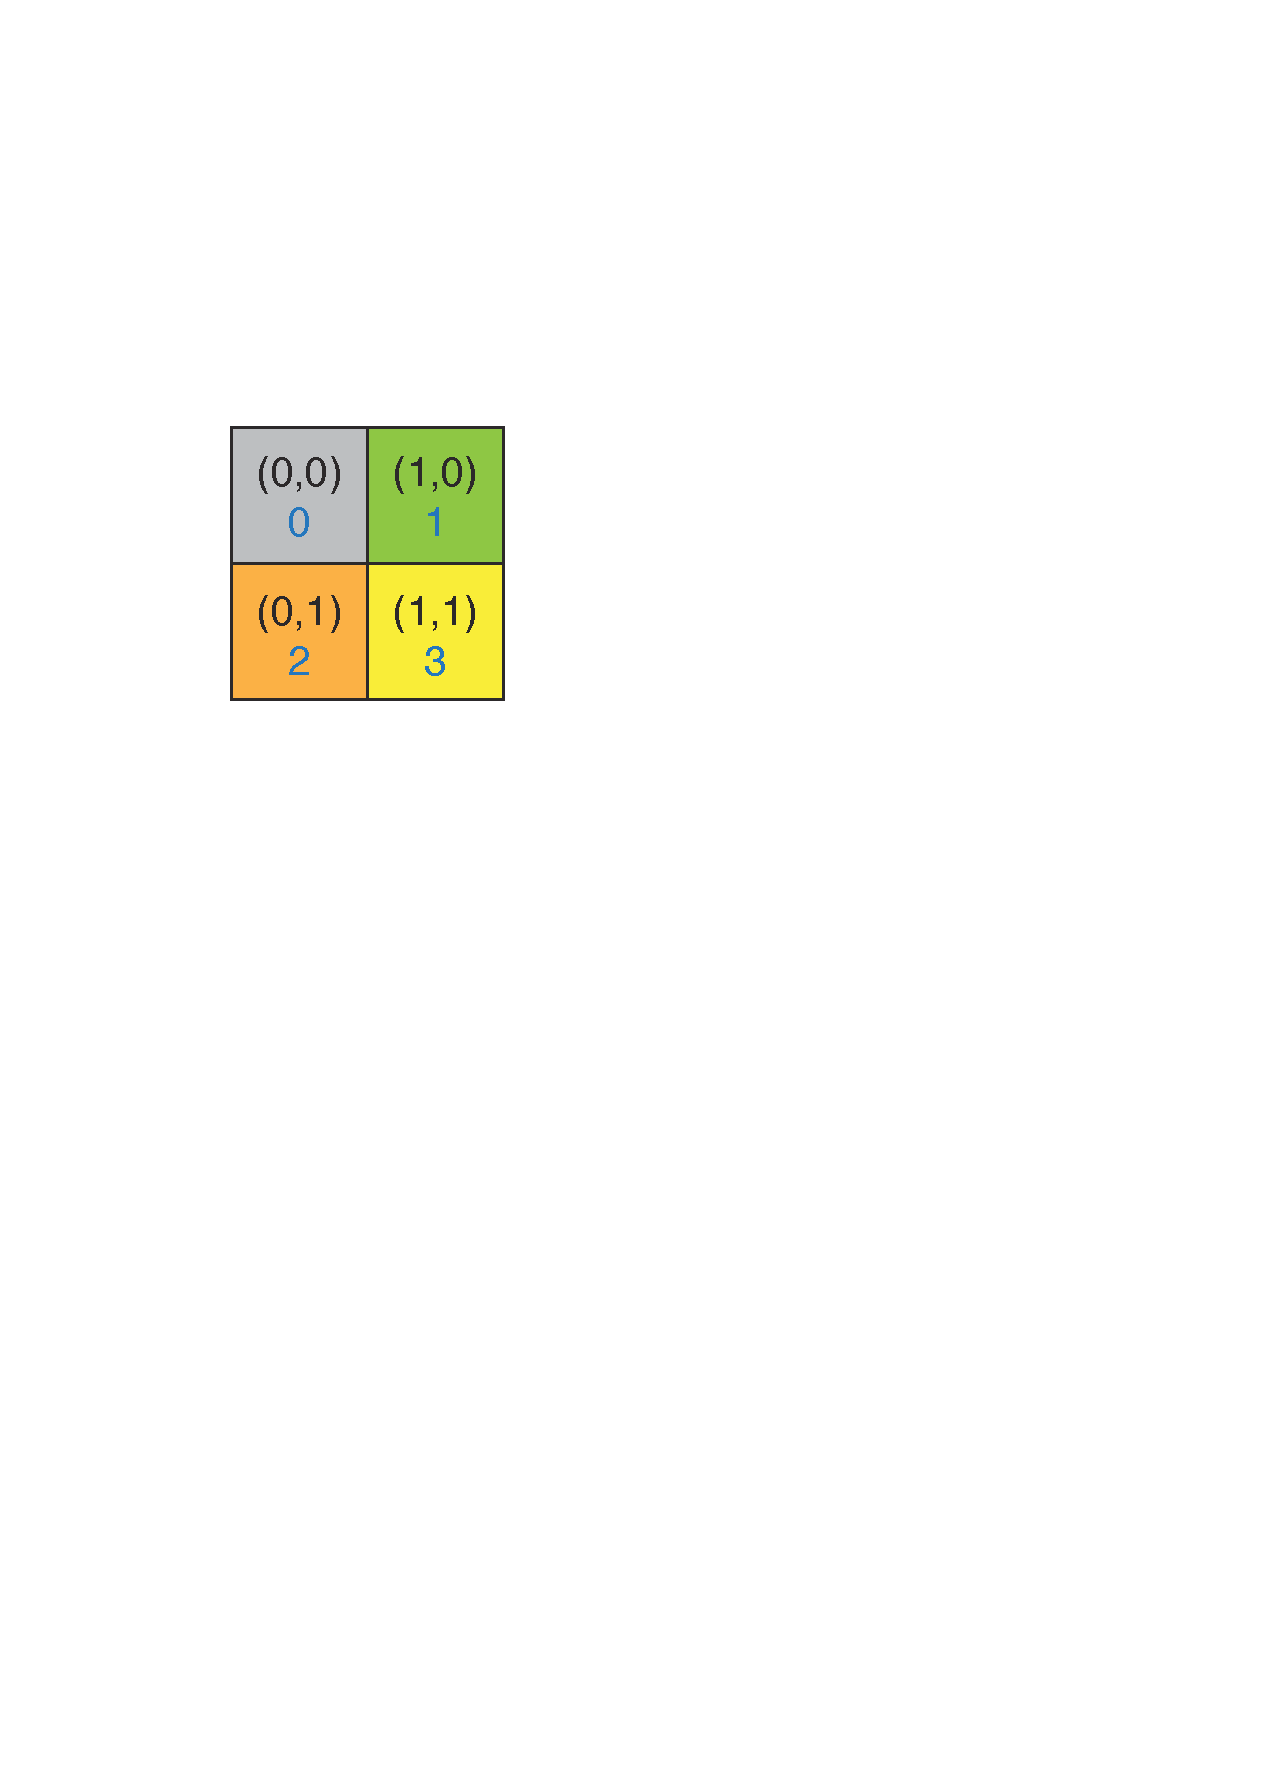
\includegraphics[height=0.25\textheight]{figure/grid-row-major.pdf}
\caption{row-major}
\label{fig:winter}
\end{center}
\end{minipage}
\begin{minipage}{0.4\hsize}
\begin{center}
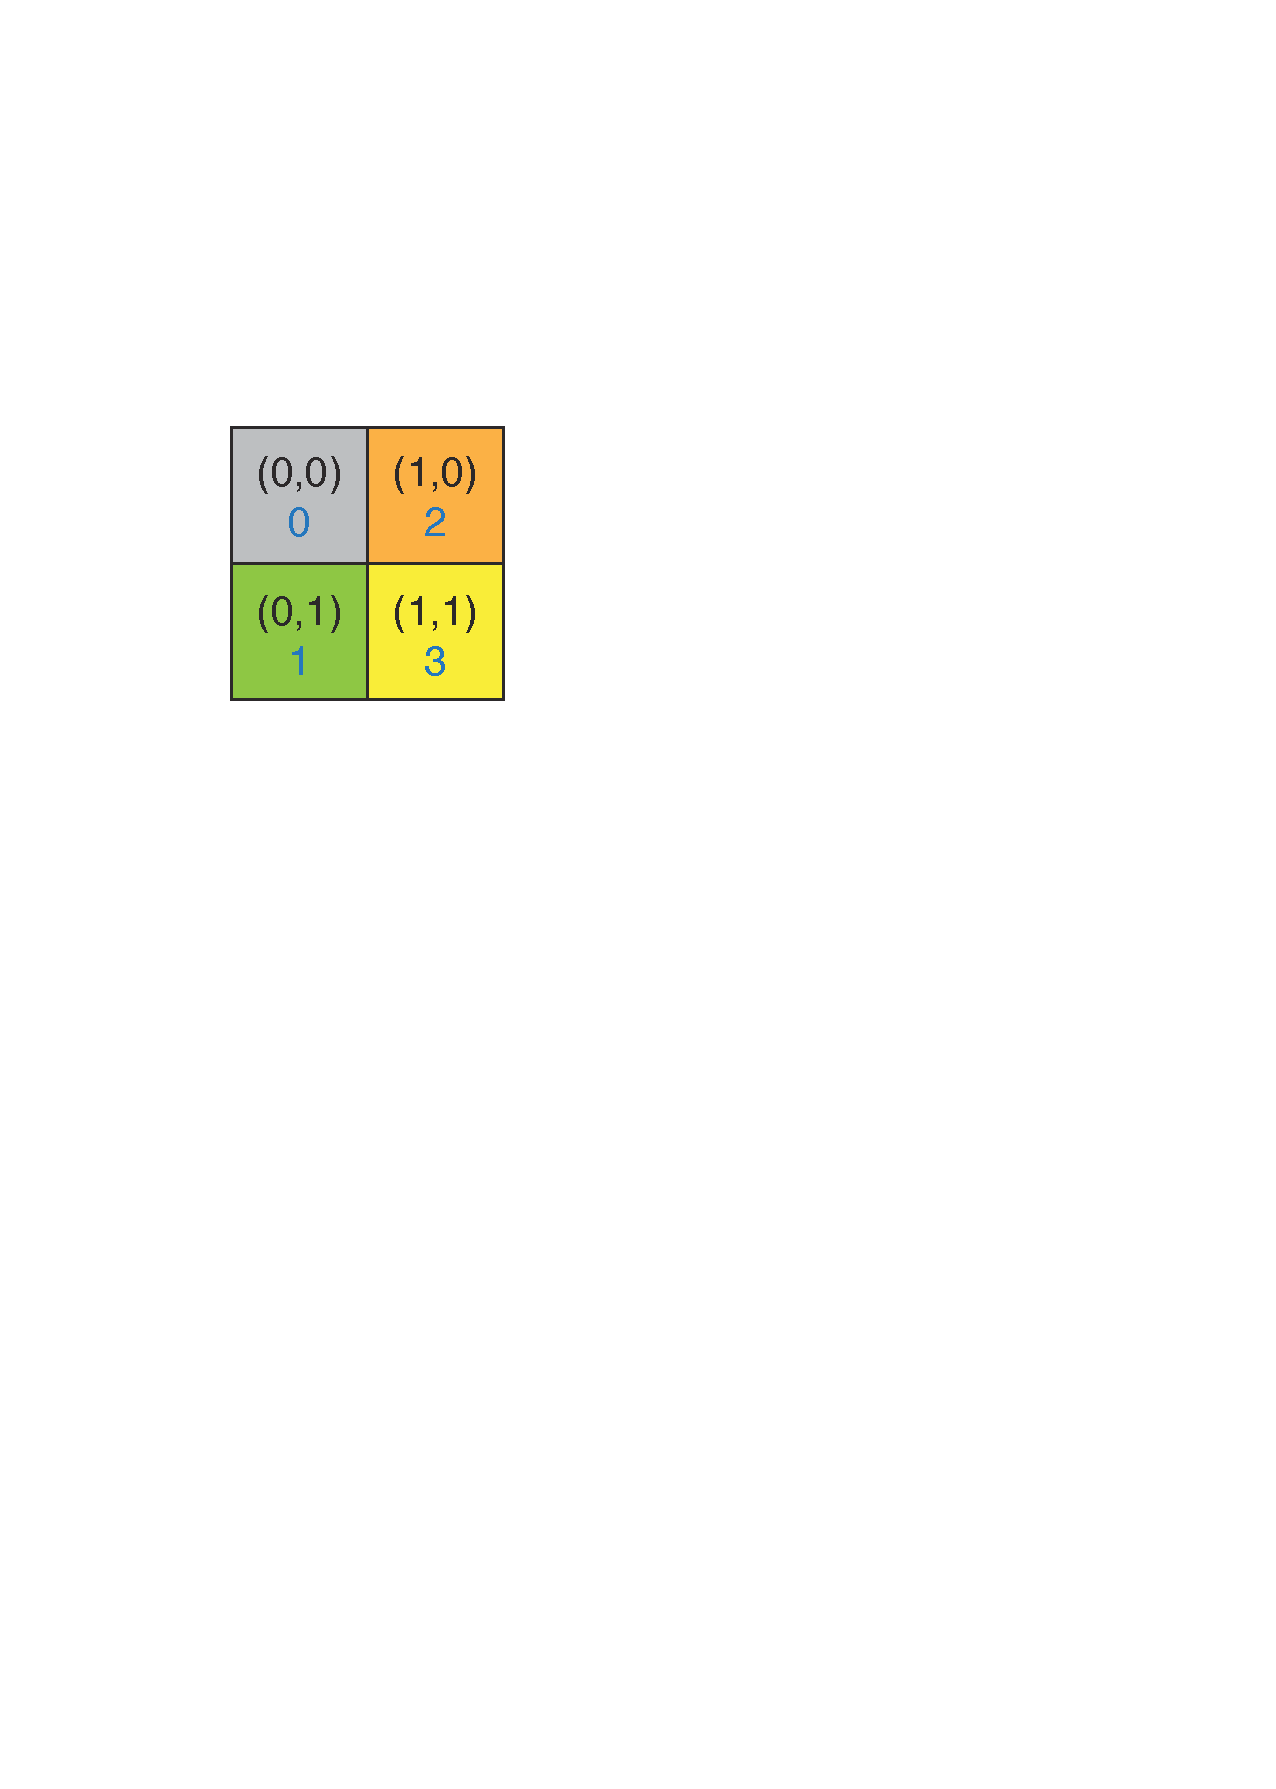
\includegraphics[height=0.25\textheight]{figure/grid-column-major.pdf}
\caption{column-major}
\label{fig:fall}
\end{center}
\end{minipage}
\end{tabular}
\end{figure}
  \item All dense solvers support both grid majors.
  \end{itemize}
\end{frame}

\begin{frame}
  \frametitle{2-dimensional block cyclic matrix (distributed_matrix)}
  \begin{itemize}
    %\setlength{\itemsep}{1em}
  \item Parallel linear algebra libraries for dense matrices employ 2D process grid.
  \item Example (using the 2D process grid in the last page):(left:local view, right:global view)
  \begin{center}
    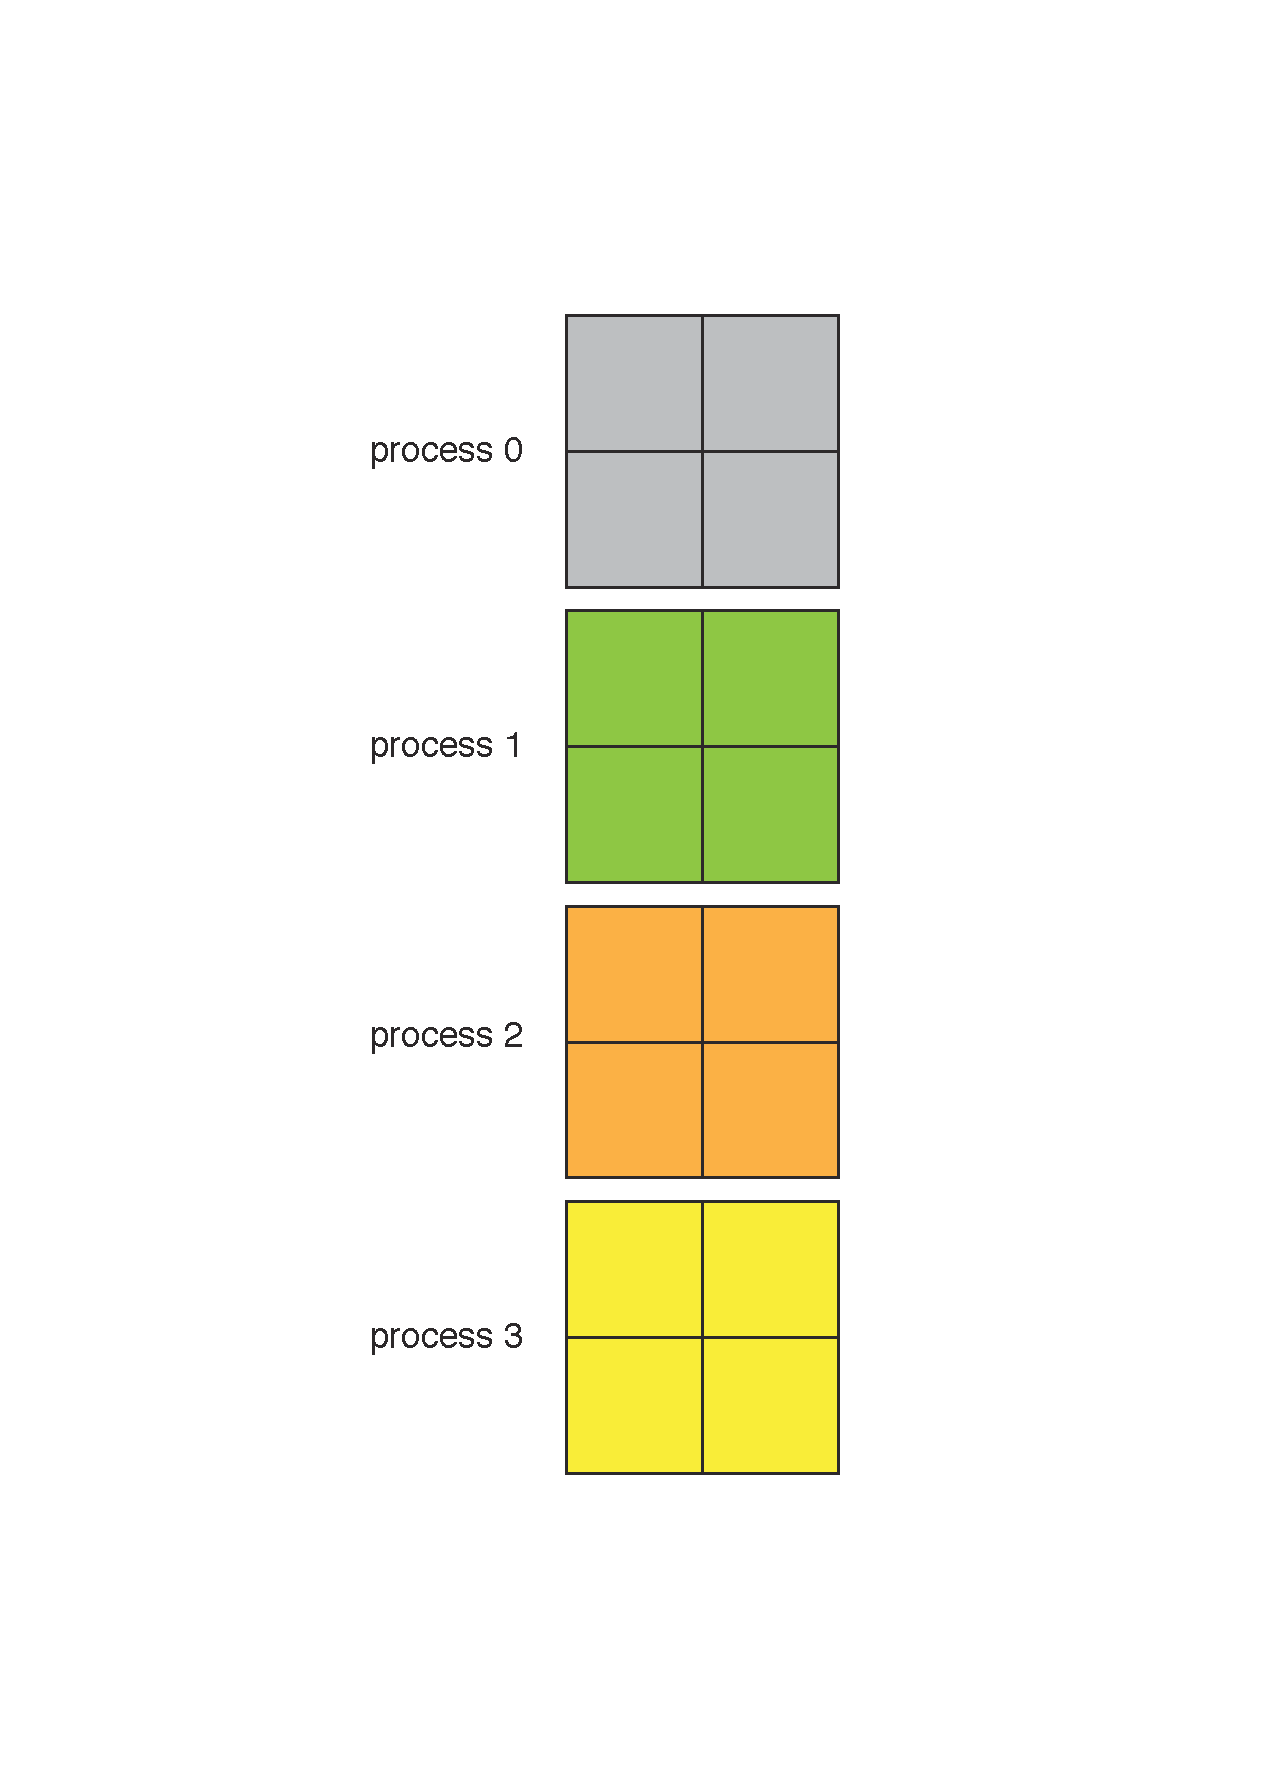
\includegraphics[height=0.45\textheight]{figure/local-view.pdf} \ \ \ \ \ \ \ \
    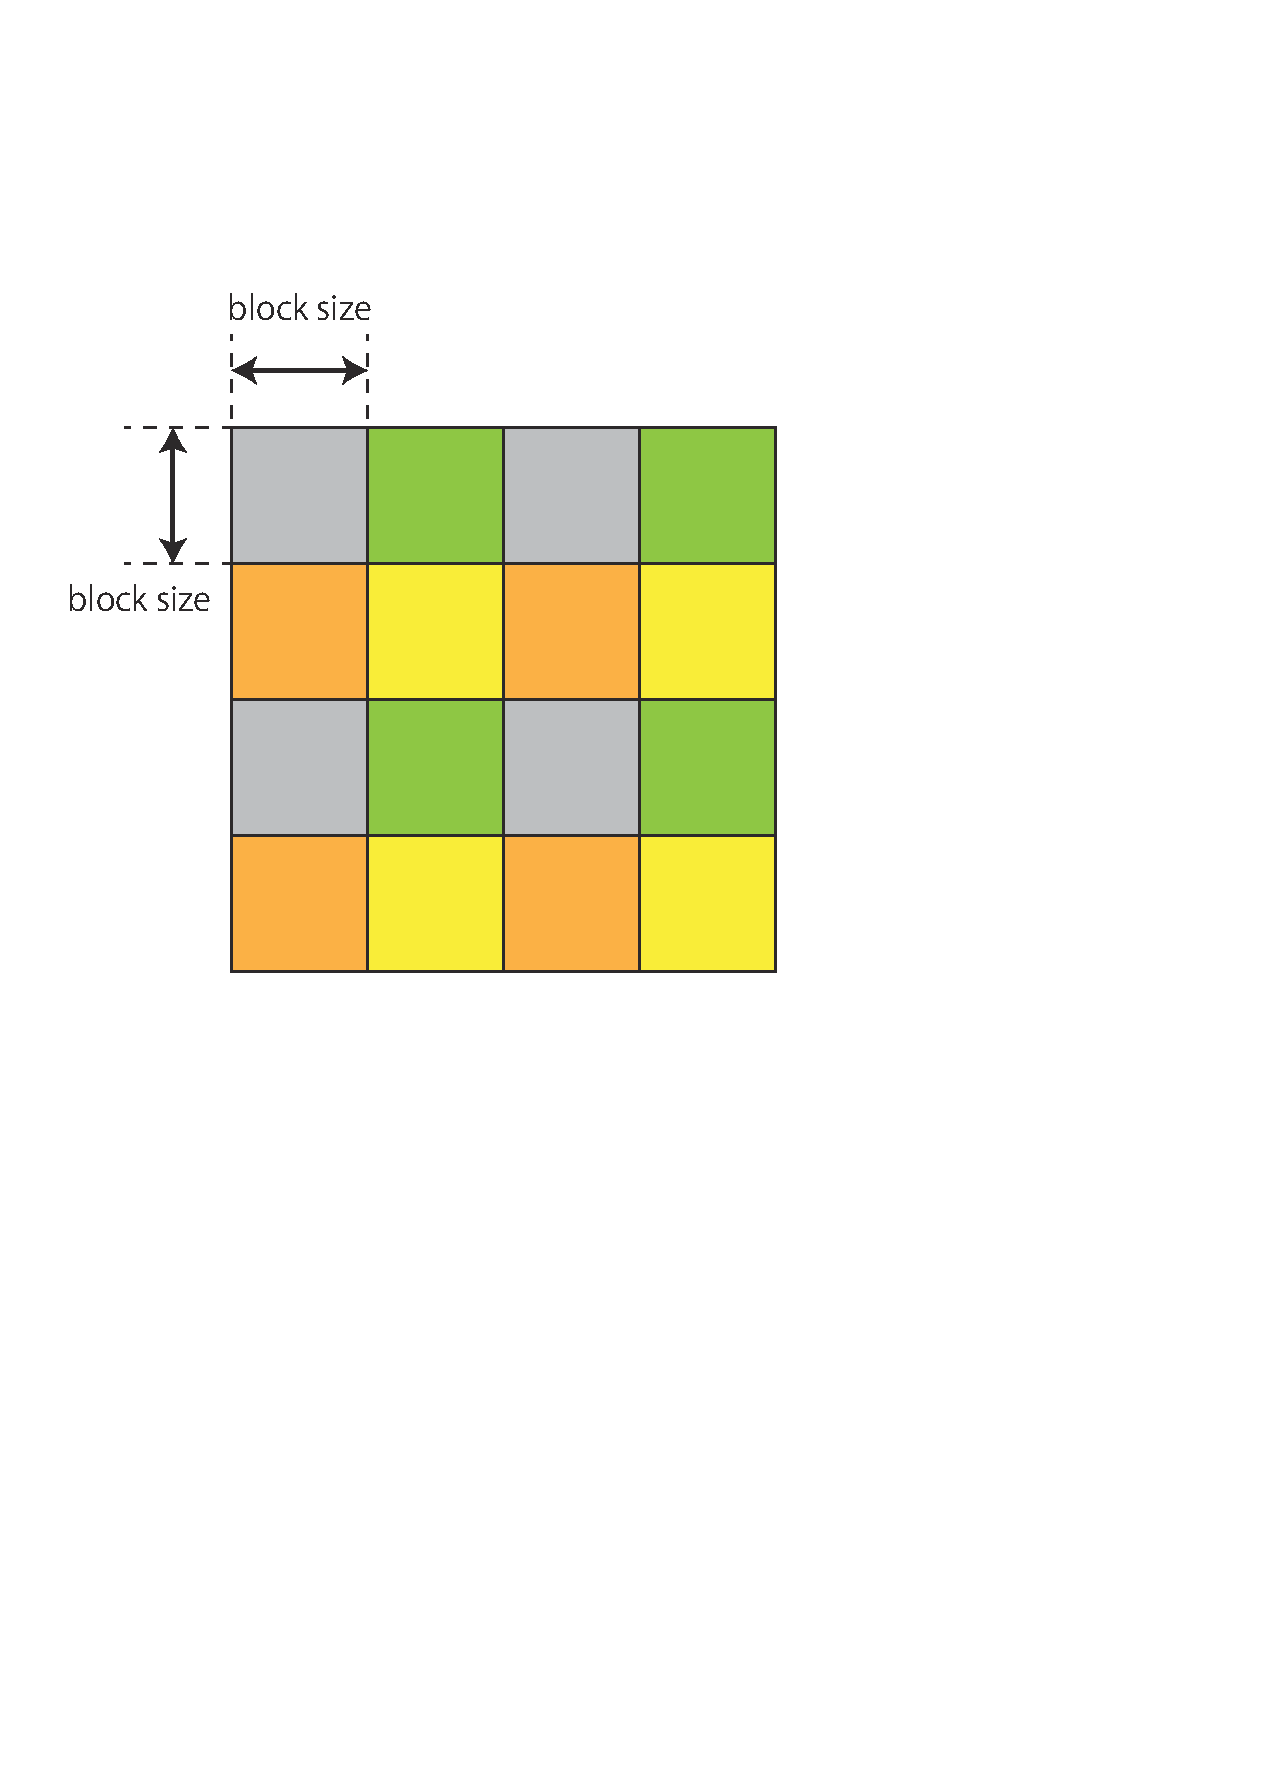
\includegraphics[height=0.35\textheight]{figure/global-view.pdf}
  \end{center}
  \item ScaLAPACK and ELPA support arabitrary block sizes.
  \item EigenExa and Elemental support $1 \times 1$.
  \end{itemize}
\end{frame}

\subsection{Specification of Rokko interface}

\begin{frame}[c,fragile]
  \frametitle{rokko::grid class}
  \begin{itemize}
  \item \RokkoFilename{rokko/grid.hpp}
\begin{lstlisting}
namespace rokko {
extern struct grid_row_major_t {} grid_row_major;
extern struct grid_col_major_t {} grid_col_major;
class grid {
public:
  explicit grid(MPI_Comm comm_in = MPI_COMM_WORLD);
  template <typename GRID_MAJOR>
  grid(MPI_Comm comm_in, GRID_MAJOR const& grid_major);
  MPI_Comm get_comm() const { return comm; }
  int get_nprocs() const;
  int get_nprow() const;
  int get_npcol() const;
  int get_myrank() const;
  int get_myrow() const;
  int get_mycol() const;
  bool is_row_major() const;
  bool is_col_major() const;
  int calculate_grid_row(int proc_rank) const;
  int calculate_grid_col(int proc_rank) const;
};
}
\end{lstlisting}
  \end{itemize}
\end{frame}


\begin{frame}[c,fragile]
  \frametitle{rokko::distributed_matrix class template}
  \begin{itemize}
  \item \RokkoFilename{rokko/distributed_matrix.hpp}
\begin{lstlisting}
namespace rokko {
template<typename MATRIX_MAJOR = rokko::matrix_row_major>
class distributed_matrix {
public:
  template<typename SOLVER>
  distributed_matrix(int m_global_in, int n_global_in, const grid& g_in, SOLVER const& solver_in);
  template<typename SOLVER>
  void initialize(int m_global_in, int n_global_in, const grid& g_in, SOLVER const& solver_in);
  int get_mb() const;
  int get_nb() const;
  int get_nprow() const;
  ...
  bool is_gindex_myrow(const int& global_i) const;
  bool is_gindex_mycol(const int& global_j) const;
  bool is_gindex(const int& global_i, const int& global_j) const;
  void set_local(int local_i, int local_j, double value);
  double get_local(int local_i, int local_j) const;
  void update_local(int local_i, int local_j, double value);
  void set_global(int global_i, int global_j, double value);
  double get_global(int global_i, int global_j) const;
};
}
\end{lstlisting}
  \end{itemize}
\end{frame}

\begin{frame}[c,fragile]
  \frametitle{Operation for distributed_matrix}
  \begin{itemize}
    %\setlength{\itemsep}{1em}
  \item Matrix-matrix product $C = \alpha A B + \beta C$
\begin{lstlisting}
  ...
  rokko::distributed_matrix<rokko::matrix_col_major> matA(dim, dim, g, solver);
  rokko::distributed_matrix<rokko::matrix_col_major> matB(dim, dim, g, solver);
  rokko::distributed_matrix<rokko::matrix_col_major> matC(dim, dim, g, solver);
  ...
  rokko::product(alpha, matA, transA, matB, transB, beta, matC);
\end{lstlisting}
  \item Scatter \& Gather for distributed_matrix
\begin{lstlisting}
  rokko::localized_matrix<LOC_MAT_MAJOR> lmat(dim, dim);
  rokko::distributed_matrix<DIST_MAT_MAJOR> mat(dim, dim, g, solver);
  rokko::scatter(lmat, mat, root);
  rokko::gather(mat, lmat, root);
\end{lstlisting}
  \end{itemize}
\end{frame}

\begin{frame}[c,fragile]
  \frametitle{generating distributed_matrix}
  \begin{itemize}
    %\setlength{\itemsep}{1em}
  \item assign matrix elements (global indices)
\begin{lstlisting}
for(int global_i=0; global_i < mat.m_global; ++global_i) {
  for(int global_j=0; global_j < mat.n_global; ++global_j) {
    mat.set_global(global_i, global_j, f(global_i, global_j));
  }
}
\end{lstlisting}
  \item assign matrix elements (local indices)
\begin{lstlisting}
for(int local_i = 0; local_i < mat.get_m_local(); ++local_i) {
  for(int local_j = 0; local_j < mat.get_n_local(); ++local_j) {
    int global_i = mat.translate_l2g_row(local_i);
    int global_j = mat.translate_l2g_col(local_j);
    mat.set_local(local_i, local_j, f(global_i, global_j));
  }
}
\end{lstlisting}
  \item generate all matrix elements by function
\begin{lstlisting}
mat.generate(f);
\end{lstlisting}
  \end{itemize}
\end{frame}

\begin{frame}[c,fragile]
  \frametitle{rokko::parallel_dense_solver class}
  \begin{itemize}
    %\setlength{\itemsep}{1em}
  \item Initialize solver
\begin{lstlisting}
rokko::parallel_dense_solver solver(name);
solver.initialize(argc, argv);
\end{lstlisting}
  \item Finalize solver
\begin{lstlisting}
solver.finalize();
\end{lstlisting}
  \item Diagonalize a matrix (the matrix is overwrriten)
\begin{lstlisting}
rokko::distributed_matrix<matrix_col_major> mat(dim, dim, g, solver);
...
rokko::localized_vector evals(dim);
rokko::distributed_matrix<matrix_col_major> evecs(dim, dim, g, solver);
solver.diagonalize(mat, evals, evecs);
\end{lstlisting}
%  \item 登録されているソルバの一覧
%\begin{lstlisting}
%std::vector<std::string> names = rokko::parallel_dense_solver::solvers();
%\end{lstlisting}
  \end{itemize}
\end{frame}

\subsection{Run sample}

\begin{frame}[c,fragile]
  \frametitle{Sample programs for diagonalization}
  \begin{itemize}
    %\setlength{\itemsep}{1em}
%  \item MPI並列密行列ソルバーの一覧 \href{https://github.com/t-sakashita/rokko/blob/master/test/parallel_dense_solvers.cpp}{test/parallel\_dense\_solvers.cpp}
%\begin{lstlisting}[style=shstyle]
%./test/parallel_dense_solvers
%\end{lstlisting}
  \item C++ \RokkoFilename{sample/dense/frank_mpi.cpp}
\begin{lstlisting}[style=shstyle]
mpirun -np 4 ./sample/dense/frank_mpi eigen_exa_sx 5
\end{lstlisting}
  \item C \RokkoFilename{sample/dense/frank_mpi.cpp}
\begin{lstlisting}[style=shstyle]
mpirun -np 4 ./sample_c/dense/frank_mpi eigen_exa_sx 5
\end{lstlisting}
  \item Fortran \RokkoFilename{sample/dense/frank_mpi.cpp}
\begin{lstlisting}[style=shstyle]
mpirun -np 4 ./sample_fortran/dense/frank_mpi eigen_exa_sx 5
\end{lstlisting}

  \end{itemize}
\end{frame}

\begin{frame}[c,fragile]
  \frametitle{Test matrix: Frank matrix (definition)}
\begin{block}{Definition}
$[a_{ij}]_{i,j = {0, \dots, n-1}} = [ n - \max(i,j) ]$\\
\end{block}

\begin{block}{Example ($n=5$)}
$[a_{ij}]_{i,j = {0, \dots, 4}} =
\begin{bmatrix}
5 & 4 & 3 & 2 & 1 \\
4 & 4 & 3 & 2 & 1 \\
3 & 3 & 3 & 2 & 1 \\
2 & 2 & 2 & 2 & 1 \\
1 & 1 & 1 & 1 & 1 \\
\end{bmatrix}
$
\end{block}
\end{frame}

\begin{frame}[c,fragile]
  \frametitle{Test matrix: Frank matrix (properties)}
\begin{block}{Analytical eigenvalues}%
$\lambda_k = \dfrac{1}{2 \left( 1 - \cos{\tfrac{2 k + 1}{2 n + 1}\pi} \right)} \quad (k=0,\dots,n-1)$
\end{block}

\begin{block}{Remark}%
Frank matrix has an eigenvalue $1$\\
\quad $\Longleftrightarrow$ $\tfrac{2 k + 1}{2 n + 1} = \tfrac{1}{3}$\\
\quad $\Longleftrightarrow$ $n-1$ is a multiple of 3.
\end{block}
\end{frame}

\section{Parallel sparse solvers}

\subsection{Basic concepts}

\begin{frame}[c,fragile]
  \frametitle{CRS (Compressed Row Storage) format}
%疎行列の非ゼロ成分のみを求め固有値ソルバに渡す方法である.
%この方法で用いられる疎行列の代表的な格納方式には,CRS方式(Compressed Row Storage, 圧縮行格納方式)がある.
For each row, nonzero entries and their column indices are stored.

\begin{rei}%
\vspace{-2\baselineskip}
\begin{align*}
\begin{bmatrix}
7.1 & 5.2 & 0 & 0 \\
0 & 0 & 0 & 6.4 \\
0.2 & 0 & 0 & 4.3 \\
0 & 0 & 0.5 & 0
\end{bmatrix}
\end{align*}
Representation in CRS format:
\begin{itemize}
%\item 非ゼロ成分に対する行添字$= [1, 1, 2, 3, 3, 4] $
\item $nonzero\_rows = [2, 1, 2, 1]$
\item $nonzero\_cols = [1, 2, 4, 1, 4, 3]$
%\begin{bmatrix}
%1 & 2 \\
%4 \\
%1 & 4 \\
%3
%\end{bmatrix}$
\item $nonzero\_entries = [7.1, 5.2, 6.4, 0.2, 4.3, 0.5]$
\end{itemize}
\end{rei}

Parallelization can be done for rows.
This parallelization is automatically done by eigensolvers.

\end{frame}

\subsection{Specifications for Rokko interfaces}

\begin{frame}[c,fragile]
  \frametitle{rokko::distributed_crs_matrix class template}
  \begin{itemize}
  \item \RokkoFilename{rokko/distributed_crs_matrix.hpp}
\begin{lstlisting}
namespace rokko {
class distributed_crs_matrix {
public:
  template<typename SOLVER>
  distributed_crs_matrix(int row_dim, int col_dim, SOLVER& solver_in)
  void insert(int row, std::vector<int> const& cols, std::vector<double> const& values);
  void insert(int row, int col_size, int* cols, double* const values);
  void complete();
  int get_dim() const;
  int num_local_rows() const;
  int start_row() const;
  int end_row() const;
  void print() const;
};
}
\end{lstlisting}
  \end{itemize}
\end{frame}


\begin{frame}[c,fragile]
  \frametitle{rokko::distributed_crs_matrix class (example)}
\RokkoFilename{sample/sparse/distributed_crs_matrix.cpp}
\begin{lstlisting}
  rokko::parallel_sparse_solver solver("anasazi");
  int dim = 4;
  rokko::distributed_crs_matrix mat(dim, dim, solver);

  int num_nonzero_cols[] = {2, 1, 2, 1};
  int nonzero_cols[] = {0, 1, 3, 0, 3, 2};
  double values[] = {7.1, 5.2, 6.4, 0.2, 4.3, 0.5};

  int current = 0;
  for (int row = 0; row < dim; ++row) {
    mat.insert(row, num_nonzero_cols[row], &nonzero_cols[current], &values[current]);
    current += num_nonzero_cols[row];
  }
  mat.complete();
  mat.print();
\end{lstlisting}
\noindent
Run sample
  \begin{itemize}
  \item For using Anasazi
\begin{lstlisting}[style=shstyle]
mpirun -np 4 ./sample/sparse/distributed_crs_matrix anasazi
\end{lstlisting}
  \item For using SLEPc
\begin{lstlisting}[style=shstyle]
mpirun -np 4 ./sample/sparse/distributed_crs_matrix slepc
\end{lstlisting}
  \end{itemize}
\end{frame}


\begin{frame}[c,fragile]
  \frametitle{Matrix free method}
%たいていの疎行列向け固有値ソルバでは、行列そのものではなく、固有値分解を行うべき行列とベクトル積を行うルーチンのみが必要である。
% \\
\noindent
Write a class
  \begin{itemize}
  \item \RokkoFilename{rokko/utility/heisenberg_hamiltonian.hpp}
\begin{lstlisting}
class heisenberg_op : public rokko::distributed_mfree {
public:
  heisenberg_op(int L, const std::vector<std::pair<int, int> >& lattice) : L_(L), lattice_(lattice) {
    comm_ = MPI_COMM_WORLD;
    int nproc;
    MPI_Comm_size(comm_, &nproc);
    int n = nproc;
    int p = -1;
    do {
      n /= 2;
      ++p;
    } while (n > 0);
    local_N = 1 << (L-p);
    buffer_.assign(local_N, 0);
    dim_ = 1 << L;
  }
  void multiply(const double* x, double* y) const {
    rokko::heisenberg_hamiltonian::multiply(comm_, L_, lattice_, x, y, &(buffer_[0]));
  }
  int get_dim() const {
    return dim_;
  }
  int get_num_local_rows() const {
    return local_N;
  }
\end{lstlisting}
  \end{itemize}
\end{frame}

\begin{frame}[c,fragile]
  \frametitle{Matrix free method (cont.)}
\begin{lstlisting}
private:
  MPI_Comm comm_;
  mutable std::vector<double> buffer_;
  int L_;
  int local_N;
  std::vector<std::pair<int, int> > lattice_;
  int dim_;
};
\end{lstlisting}
\end{frame}


\begin{frame}[c,fragile]
  \frametitle{rokko::parallel_sparse_solver class}
\vspace{-1\baselineskip}
  \begin{itemize}
    %\setlength{\itemsep}{1em}
  \item Initialize solver
\begin{lstlisting}
rokko::parallel_sparse_solver solver(name);
solver.initialize(argc, argv);
\end{lstlisting}
  \item Finalize solver
\begin{lstlisting}
solver.finalize();
\end{lstlisting}
  \item Diagonalize a sparse matrix in CRS format
\begin{lstlisting}
rokko::distributed_crs_matrix mat(dim, dim, solver);
...
solver.diagonalize(mat, num_evals, block_size, max_iters, tol);
\end{lstlisting}
  \item Diagonalize MatFree
\begin{lstlisting}
heisenberg_op  mat(L, lattice);
solver.diagonalize(mat, num_evals, block_size, max_iters, tol);
\end{lstlisting}
  \item Retrieve the computed eigenvalues \& eigenvectors
\begin{lstlisting}
int i;
solver.eigenvalue(i);
std::vector<double> eigvec;
solver.eigenvector(i, eigvec);
\end{lstlisting}
%  \item 登録されているソルバの一覧
%\begin{lstlisting}
%std::vector<std::string> names = rokko::parallel_sparse_solver::solvers();
%\end{lstlisting}
  \end{itemize}
\end{frame}



\section{Diagonalization for the quantum spin system}

\begin{frame}[c,fragile]
  \frametitle{Diagonalization for the quantum spin system (dense matrix, seq. / MPI)}
  \begin{itemize}
    %\setlength{\itemsep}{1em}
  \item Heisenberg model (seq.) \RokkoFilename{sample/dense/heisenberg.cpp}
\begin{lstlisting}[style=shstyle]
./sample/dense/heisenberg lapack
\end{lstlisting}
  \item Heisenberg model (MPI) \RokkoFilename{sample/dense/heisenberg_mpi.cpp}
\begin{lstlisting}[style=shstyle]
mpirun -np 4 ./sample/dense/heisenberg_mpi eigen_exa_sx
\end{lstlisting}
  \item XYZ model (seq.) \RokkoFilename{sample/dense/xyz.cpp}
\begin{lstlisting}[style=shstyle]
./sample/dense/xyz_dense lapack $HOME/rokko-0.1/test/input_data/xyz_1hexagon.ip
\end{lstlisting}
  \item XYZ model (MPI) \RokkoFilename{sample/dense/xyz_mpi.cpp}
\begin{lstlisting}[style=shstyle]
mpirun -np 4 ./sample/dense/xyz_mpi eigen_exa_sx $HOME/rokko-0.1/test/input_data/xyz_1hexagon.ip
\end{lstlisting}
  \end{itemize}
\end{frame}

\begin{frame}[c,fragile]
  \frametitle{Diagonalization for quantum spin system (sprase matrix, MPI)}
  \begin{itemize}
    %\setlength{\itemsep}{1em}
  \item Heisenberg model(CRS) \RokkoFilename{sample/sparse/heisenberg_crs_mpi.cpp}
%\href{https://github.com/t-sakashita/rokko/blob/master/sample_anasazi/heisenberg_crs_mpi.cpp}{sample/sparse/heisenberg\_crs\_mpi.cpp}
\begin{lstlisting}[style=shstyle]
mpirun -np 4 ./sample/sparse/heisenberg_crs_mpi
\end{lstlisting}
  \item Heisenberg model(MatFree) \RokkoFilename{sample/sparse/heisenberg_mfree_mpi.cpp}
\begin{lstlisting}[style=shstyle]
mpirun -np 4 ./sample/sparse/heisenberg_mfree_mpi
\end{lstlisting}
  \item XYZ model(CRS) \RokkoFilename{sample/sparse/xyz_crs_mpi.cpp}
\begin{lstlisting}[style=shstyle]
mpirun -np 4 ./sample/sparse/xyz_crs_mpi
\end{lstlisting}
  \item XYZ model(Matfree) \RokkoFilename{sample/sparse/xyz_mfree_mpi.cpp}
\begin{lstlisting}[style=shstyle]
mpirun -np 4 ./sample/sparse/xyz_mfree_mpi
\end{lstlisting}
  \end{itemize}
\end{frame}

\section{TITPACK2へのRokko組み込み実習}

%\begin{frame}[c,fragile]
%  \frametitle{TITPACKの概要}
%\end{frame}

\begin{frame}[c,fragile]
  \frametitle{ハイゼンベルグ模型}
\setlength{\fboxsep}{1pt}

\noindent
\begin{align*}
\mathcal{H} &= J \sum\limits_{\langle j,k \rangle} {\boldmath S}_j \cdot S_k \\
&= J \sum\limits_{\langle j,k \rangle} \left\{ S^z_j S^z_k + \tfrac{1}{2}(S^+_j S^-_k + S^-_j S^+_k) \right\}
\end{align*}

\begin{align*}
\text{Here, } & S^z_j S^z_k + \tfrac{1}{2}(S^+_j S^-_k + S^-_j S^+_k) \\
 &=
\tfrac{1}{2}
\begin{bmatrix}
1 & 0 \\
0 & -1
\end{bmatrix}
\otimes
\tfrac{1}{2}
\begin{bmatrix}
1 & 0 \\
0 & -1
\end{bmatrix}
+
\tfrac{1}{2}\left\{
\begin{bmatrix}
0 & 1 \\
0 & 0
\end{bmatrix}
\otimes
\begin{bmatrix}
0 & 0 \\
1 & 0
\end{bmatrix}
+
\begin{bmatrix}
0 & 0 \\
1 & 0
\end{bmatrix}
\otimes
\begin{bmatrix}
0 & 1 \\
0 & 0
\end{bmatrix}
\right\}\\
&=
\begin{bmatrix}
\tfrac{1}{4} & & & \\
 & - \tfrac{1}{4} & \tfrac{1}{2} & \\
 & \tfrac{1}{2} & - \tfrac{1}{4} & \\
 & & & \tfrac{1}{4}
\end{bmatrix}
\end{align*}

\end{frame}

\begin{frame}[c,fragile]
  \frametitle{ディレクトリ構成}

\dirtree{%
 .1 \href{https://github.com/t-sakashita/rokko/tree/develop/tutorial/}{tutorial}.
 .2
 \href{https://github.com/t-sakashita/rokko/tree/develop/tutorial/titpack}{titpack}.
 .3
 \href{https://github.com/t-sakashita/rokko/tree/develop/tutorial/titpack/00_original}{00\_original}
 $\cdots$ 独自固有値ソルバのFortran版.
 .3
 \href{https://github.com/t-sakashita/rokko/tree/develop/tutorial/titpack/01_lapack}{01\_lapack}
 $\cdots$ FortranのままLAPACK化.
 .3
 \href{https://github.com/t-sakashita/rokko/tree/develop/tutorial/titpack/01_lapack_cxx}{01\_lapack\_cxx}
 $\cdots$ C++でLAPACK版.
 .3
 \href{https://github.com/t-sakashita/rokko/tree/develop/tutorial/titpack/02_refactored_cxx}{02\_refactored\_cxx}
 $\cdots$ C++版のリファクタリング版.
 .3
 \href{https://github.com/t-sakashita/rokko/tree/develop/tutorial/titpack/03_rokko_cxx}{03\_rokko\_cxx}
 $\cdots$ C++でRokko化.
}
\end{frame}


\section{アプリケーションからのRokkoの利用}

\begin{frame}[c,fragile]
  \frametitle{CMakeによるRokkoライブラリの取り込み方法}
以下を参考にユーザプログラム用のCMakeLists.txtを書く。

そのCMakeLists.txtにshare/rokko/UseRokko.cmakeをインクルードする。

\begin{itemize}
  \item \href{https://github.com/t-sakashita/rokko/tree/develop/sample/CMakeLists.txt}{sample/CMakeLists.txt}
  \item \href{https://github.com/t-sakashita/rokko/tree/develop/sample_c/CMakeLists.txt}{sample\_c/CMakeLists.txt}
  \item \href{https://github.com/t-sakashita/rokko/tree/develop/sample_fortran/CMakeLists.txt}{sample\_fortran/CMakeLists.txt}
\end{itemize}
\end{frame}


%\begin{frame}[c,fragile]
%  \frametitle{MakefileによるRokkoライブラリの取り込み方法}
ユーザプログラムのMakefileにshare/rokko/include.mkをインクルードする。

%\end{frame}


\end{document}




%\section{ALPS/Baristaパッケージ}
%\section{MateriAppsとMateriApps LIVE!}

\begin{frame}
  \frametitle{テスト}
  \begin{itemize}
    %\setlength{\itemsep}{1em}
  \item テスト
  \end{itemize}
\end{frame}

